\documentclass[10pt,border=1pt]{standalone}
\usepackage[T1]{fontenc}
\usepackage{mathpazo}
\usepackage{amsmath,amssymb}
\usepackage{xcolor}
\usepackage{pgfplots}
\pgfplotsset{compat=1.18}
\usetikzlibrary{shapes.geometric,positioning,arrows.meta,calc}
\definecolor{okorange}{HTML}{E69F00}
\definecolor{oksky}{HTML}{56B4E9}
\definecolor{okgreen}{HTML}{009E73}
\definecolor{okblue}{HTML}{0072B2}
\definecolor{okverm}{HTML}{D55E00}
\definecolor{okpurple}{HTML}{CC79A7}
\colorlet{accent}{okverm}
\pgfplotsset{
  safenest/.style={
    tick label style={font=\footnotesize},
    label style={font=\small},
    title style={font=\small, align=left},
    legend style={font=\footnotesize, draw=none, fill=none, cells={anchor=west}},
    grid style={black!12, line width=0.3pt},
    axis line style={black!70, line width=0.4pt},
    tick style={black!70, line width=0.4pt},
    axis lines*=left,
  },
}
\newlength{\figwidth}
\tikzset{every node/.append style={execute at begin node={\hyphenpenalty=10000\exhyphenpenalty=10000\relax}}}
\setlength{\figwidth}{13.86cm}
\begin{document}
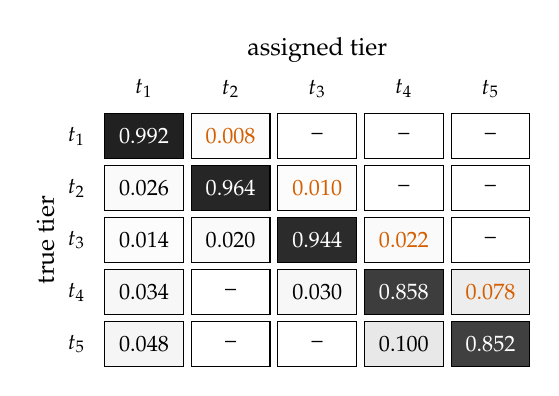
\begin{tikzpicture}[cc/.style={draw, thin, rectangle, minimum width=10mm,
                    minimum height=5.8mm, font=\footnotesize}]
\node[font=\footnotesize] at (0.00,0.6) {$t_1$};
\node[font=\footnotesize] at (1.10,0.6) {$t_2$};
\node[font=\footnotesize] at (2.20,0.6) {$t_3$};
\node[font=\footnotesize] at (3.30,0.6) {$t_4$};
\node[font=\footnotesize] at (4.40,0.6) {$t_5$};
\node[font=\footnotesize, anchor=east] at (-0.62,-0.00) {$t_1$};
\node[font=\footnotesize, anchor=east] at (-0.62,-0.66) {$t_2$};
\node[font=\footnotesize, anchor=east] at (-0.62,-1.32) {$t_3$};
\node[font=\footnotesize, anchor=east] at (-0.62,-1.98) {$t_4$};
\node[font=\footnotesize, anchor=east] at (-0.62,-2.64) {$t_5$};
\node[cc, fill=black!87, text=white] at (0.00,-0.00) {0.992};
\node[cc, fill=black!1, text=accent] at (1.10,-0.00) {0.008};
\node[cc, fill=black!0, text=black] at (2.20,-0.00) {--};
\node[cc, fill=black!0, text=black] at (3.30,-0.00) {--};
\node[cc, fill=black!0, text=black] at (4.40,-0.00) {--};
\node[cc, fill=black!2, text=black] at (0.00,-0.66) {0.026};
\node[cc, fill=black!85, text=white] at (1.10,-0.66) {0.964};
\node[cc, fill=black!1, text=accent] at (2.20,-0.66) {0.010};
\node[cc, fill=black!0, text=black] at (3.30,-0.66) {--};
\node[cc, fill=black!0, text=black] at (4.40,-0.66) {--};
\node[cc, fill=black!1, text=black] at (0.00,-1.32) {0.014};
\node[cc, fill=black!2, text=black] at (1.10,-1.32) {0.020};
\node[cc, fill=black!83, text=white] at (2.20,-1.32) {0.944};
\node[cc, fill=black!2, text=accent] at (3.30,-1.32) {0.022};
\node[cc, fill=black!0, text=black] at (4.40,-1.32) {--};
\node[cc, fill=black!3, text=black] at (0.00,-1.98) {0.034};
\node[cc, fill=black!0, text=black] at (1.10,-1.98) {--};
\node[cc, fill=black!3, text=black] at (2.20,-1.98) {0.030};
\node[cc, fill=black!76, text=white] at (3.30,-1.98) {0.858};
\node[cc, fill=black!7, text=accent] at (4.40,-1.98) {0.078};
\node[cc, fill=black!4, text=black] at (0.00,-2.64) {0.048};
\node[cc, fill=black!0, text=black] at (1.10,-2.64) {--};
\node[cc, fill=black!0, text=black] at (2.20,-2.64) {--};
\node[cc, fill=black!9, text=black] at (3.30,-2.64) {0.100};
\node[cc, fill=black!75, text=white] at (4.40,-2.64) {0.852};
\node[font=\small] at (2.2,1.1) {assigned tier};
\node[font=\small, rotate=90] at (-1.25,-1.32) {true tier};
\end{tikzpicture}
\end{document}
